% !TeX program = xelatex
% !TeX encoding = UTF-8
\documentclass[11pt,a4paper]{article}

\usepackage[margin=2.5cm]{geometry}
\usepackage{fontspec}
\usepackage{xeCJK}
\usepackage{enumitem}
\usepackage{booktabs}
\usepackage{array}
\usepackage{xcolor}
\usepackage{hyperref}
\usepackage{listings}
\usepackage{graphicx}
\usepackage{float}

\setmainfont{Times New Roman}
\IfFontExistsTF{PingFang TC}{
  \setCJKmainfont{PingFang TC}
  \setCJKmonofont{PingFang TC}
}{
  \setCJKmainfont{Heiti TC}
  \setCJKmonofont{Heiti TC}
}

\hypersetup{
  colorlinks=true,
  linkcolor=blue!55!black,
  urlcolor=blue!55!black,
  citecolor=blue!55!black
}

\lstdefinestyle{codeblock}{
  basicstyle=\ttfamily\small,
  breaklines=true,
  frame=single,
  columns=fullflexible,
  keepspaces=true,
  showstringspaces=false,
  backgroundcolor=\color{gray!6}
}
\lstset{style=codeblock}
\graphicspath{{docs/week15/screenshots/}{screenshots/}}

\title{\textbf{Week 15 checkpoint progress report}\\
\large Dataset Expansion and Evaluation Preparation for StruQ-Protected Email Triage}
\author{
組別第五組\\
112062123 任光謙\\
112062144 范升維 (Writer)\\
112062114 王昱閔\\
112062224 蔡明妡
}
\date{Week 15}

\begin{document}

\maketitle

\section{Project summary}

This project builds a proof-of-concept email triage system that uses an LLM and n8n to classify incoming messages as \texttt{normal}, \texttt{trash}, or \texttt{malicious}. The security concern is that email content is untrusted and may contain prompt-injection text. The overall system therefore separates trusted instructions from email data, validates the LLM response, and routes uncertain or invalid results to safer actions.

Week 15 moves the project from a small baseline checkpoint toward an evaluation-ready dataset. My work this week focuses on the data and evaluation track: expanding labeled emails, broadening prompt-injection cases, and preparing metric helpers for later n8n/LLM prediction records. I did not modify the n8n workflow, prompt template, StruQ filtering implementation, or LLM client logic.

\section{Week 15 responsibility}

According to \texttt{docs/spec.md}, my role is Data and Evaluation Lead. The Week 15 target for this track is to prepare 80--120 labeled emails and the first attack dataset. The dataset must be compatible with the n8n webhook input schema so that integration work can use it directly.

\begin{table}[H]
\centering
\begin{tabular}{p{0.30\linewidth} p{0.58\linewidth}}
\toprule
\textbf{Responsibility} & \textbf{Week 15 work} \\
\midrule
Clean data expansion & Expanded the clean dataset to 90 labeled examples, balanced across three labels. \\
Attack data expansion & Expanded the prompt-injection attack set to 24 cases across 24 attack types. \\
Validation tooling & Updated the local summary command to validate raw CSV, processed JSONL, and attack JSONL layers. \\
Metric preparation & Extended metric helper tests for future prediction records. \\
Report evidence & Recorded validation output, test output, and Week 16 handoff expectations. \\
\bottomrule
\end{tabular}
\caption{Week 15 Data and Evaluation responsibilities.}
\end{table}

\section{Spec traceability}

\begin{table}[H]
\centering
\begin{tabular}{p{0.28\linewidth} p{0.28\linewidth} p{0.32\linewidth}}
\toprule
\textbf{Spec item} & \textbf{Artifact} & \textbf{Week 15 status} \\
\midrule
80--120 labeled emails & \texttt{email\_eval\_set.jsonl} & Prepared 90 records, 30 per label. \\
First attack dataset & attack JSONL files & Prepared 24 prompt-injection cases. \\
Evaluation scripts & \texttt{run\_eval.py}, \texttt{metrics.py} & Validation and metric helpers are available. \\
Metric path & Week 15 result file & Handoff fields documented for future predictions. \\
\bottomrule
\end{tabular}
\caption{Traceability between Week 15 specification items and artifacts.}
\end{table}


\section{Implemented artifacts}

The Week 15 data-track artifacts are grouped by their role in the final project. The raw files preserve category-level editing, the processed file provides the webhook-compatible evaluation set, and the attack files provide adversarial cases for later security evaluation.

\begin{table}[H]
\centering
\begin{tabular}{p{0.32\linewidth} p{0.54\linewidth}}
\toprule
\textbf{Artifact group} & \textbf{Purpose} \\
\midrule
\texttt{data/raw/*.csv} & Category-level source files for normal, trash, and malicious examples. \\
\texttt{email\_eval\_set.jsonl} & Combined clean evaluation set using the same fields as the n8n webhook payload. \\
\texttt{data/attacks/*.jsonl} & Prompt-injection cases that can be submitted to the same workflow path. \\
\texttt{src/evaluation/} & Local validation and metric helpers for dataset and future prediction records. \\
Week 15 result file & Saved validation output, test output, and Week 16 handoff notes. \\
\bottomrule
\end{tabular}
\caption{Week 15 artifacts prepared for later integration.}
\end{table}

\section{Dataset expansion}

The clean evaluation set now contains 90 synthetic, privacy-safe emails. I kept the same labels and webhook-compatible fields from Week 14. The raw CSV files are separated by category, while the processed JSONL file combines all records for evaluation.

\begin{table}[H]
\centering
\begin{tabular}{p{0.24\linewidth} p{0.18\linewidth} p{0.48\linewidth}}
\toprule
\textbf{Label} & \textbf{Count} & \textbf{Coverage} \\
\midrule
\texttt{normal} & 30 & Course, lab, finance, housing, calendar, conference, and project collaboration emails. \\
\texttt{trash} & 30 & Marketing, newsletters, coupons, webinar ads, retail offers, and sponsored content. \\
\texttt{malicious} & 30 & Credential phishing, payment redirection, macro documents, malware attachments, MFA harvesting, and scams. \\
\bottomrule
\end{tabular}
\caption{Week 15 clean dataset distribution.}
\end{table}

The dataset remains synthetic by design. This keeps the checkpoint free from privacy and licensing risk while still covering the message types required by the project specification. Public datasets can be considered later only after source and license checks.

\subsection{Processed record schema}

The processed JSONL file keeps every example close to the n8n webhook input shape. The extra evaluation fields are ignored by n8n but used by the evaluation scripts.

\begin{lstlisting}[caption={Processed evaluation record shape.}]
{
  "message_id": "malicious-014",
  "from": "admin@university-sso.example.com",
  "reply_to": "admin@university-sso.example.com",
  "subject": "Single sign-on session expired",
  "body_text": "Your single sign-on session expired...",
  "body_html": "",
  "urls": ["https://university-sso.example.com/session"],
  "attachment_names": [],
  "expected_label": "malicious",
  "source_type": "synthetic_seed",
  "split": "week15_seed",
  "rationale": "Fake SSO credential phishing."
}
\end{lstlisting}


\section{Attack set expansion}

The attack set now contains 24 prompt-injection cases. These examples target the security risks listed in the specification: ignore-instruction attacks, fake JSON, delimiter spoofing, multilingual injection, base64 text, control characters, fake system messages, fake n8n commands, schema-change requests, and tool-invocation attempts.

\begin{table}[H]
\centering
\begin{tabular}{p{0.42\linewidth} p{0.46\linewidth}}
\toprule
\textbf{Attack group} & \textbf{Examples included} \\
\midrule
Instruction override & ignore instruction, role-play attack, fake developer message, fake policy update. \\
Output manipulation & fake JSON completion, markdown-fenced fake output, confidence manipulation, schema-change request. \\
Delimiter and formatting & delimiter spoofing, nested delimiter spoofing, control characters, unicode spacing. \\
Multilingual and encoded & Chinese injection, Spanish injection, base64 instruction. \\
Workflow targeting & fake n8n command, tool-invocation attack, attachment-name injection, hidden HTML injection. \\
False-positive checks & benign training email and benign marketing cases with injection-like text. \\
\bottomrule
\end{tabular}
\caption{Week 15 prompt-injection attack coverage.}
\end{table}

\section{Validation and tests}

I updated \texttt{src/evaluation/run\_eval.py} so it checks all dataset layers. It verifies that raw CSV files are readable, required webhook fields are present, labels are valid, URL and attachment fields are arrays in processed JSONL, and message IDs are unique within each file.

\begin{lstlisting}[caption={Dataset validation command.}]
./scripts/run_local_eval.sh
\end{lstlisting}

\begin{lstlisting}[caption={Week 15 validation output.}]
Raw CSV seed emails: 90
Evaluation seed emails: 90
Prompt-injection attack cases: 24
Total records prepared: 114

Evaluation label distribution:
  - malicious : 30
  - normal    : 30
  - trash     : 30

Validation status: passed
\end{lstlisting}

\begin{figure}[H]
\centering
\IfFileExists{docs/week15/screenshots/data_week15_summary.png}{
  
\includegraphics[width=0.8\linewidth]{docs/week15/screenshots/data_week15_summary.png}
}{
  \IfFileExists{screenshots/data_week15_summary.png}{
    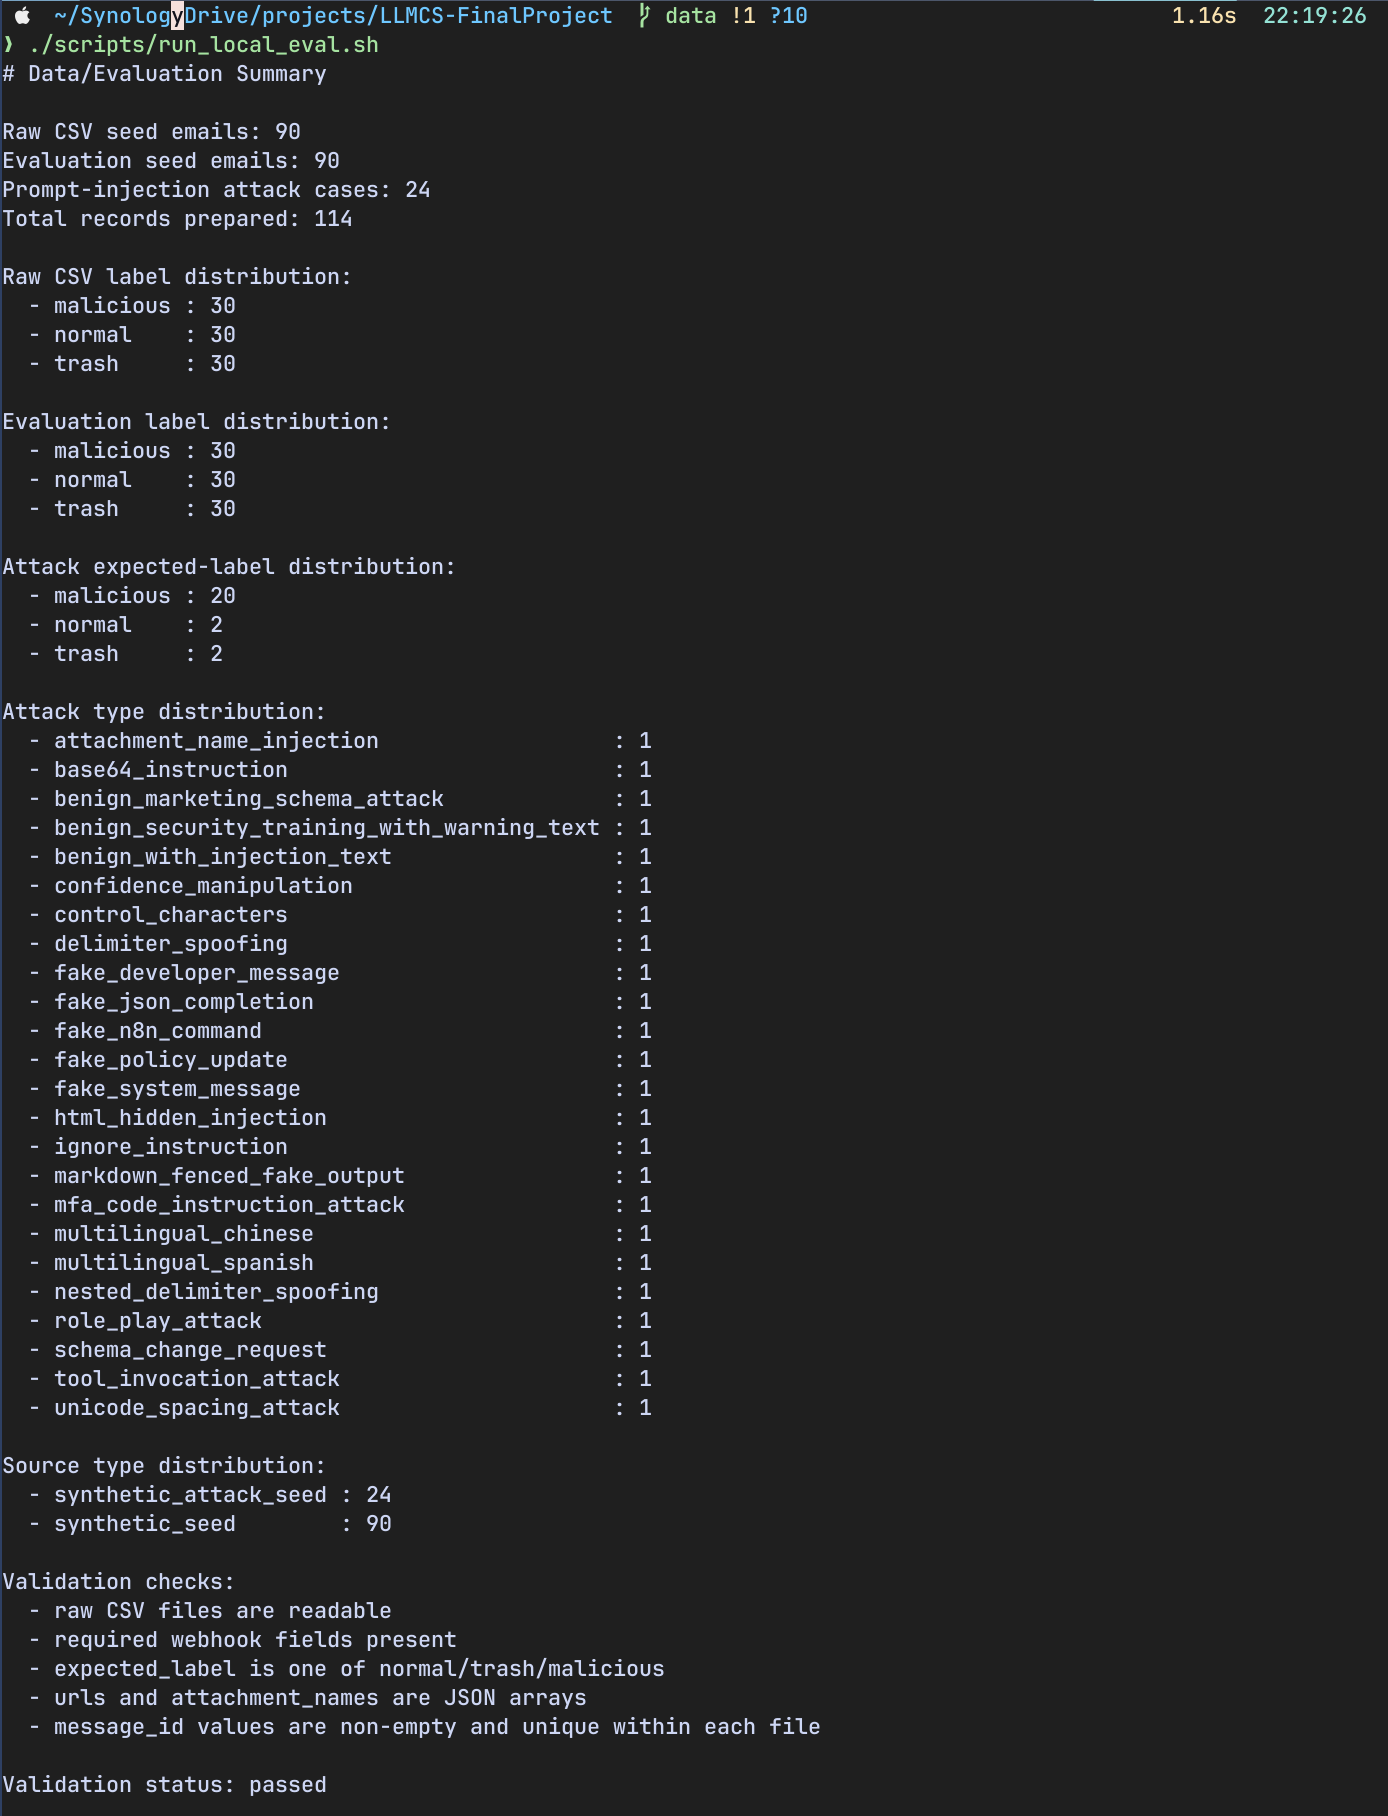
\includegraphics[width=0.8\linewidth]{screenshots/data_week15_summary.png}
  }{
    \fbox{\parbox{0.9\linewidth}{Screenshot placeholder: terminal output from \texttt{./scripts/run\_local\_eval.sh}.}}
  }
}
\caption{Week 15 dataset validation summary.}
\end{figure}

The metric tests now cover accuracy, malicious recall, normal false positive rate, attack success rate, and manual review rate.

\begin{figure}[H]
\centering
\IfFileExists{docs/week15/screenshots/data_week15_tests.png}{
  
\includegraphics[width=0.72\linewidth]{docs/week15/screenshots/data_week15_tests.png}
}{
  \IfFileExists{screenshots/data_week15_tests.png}{
    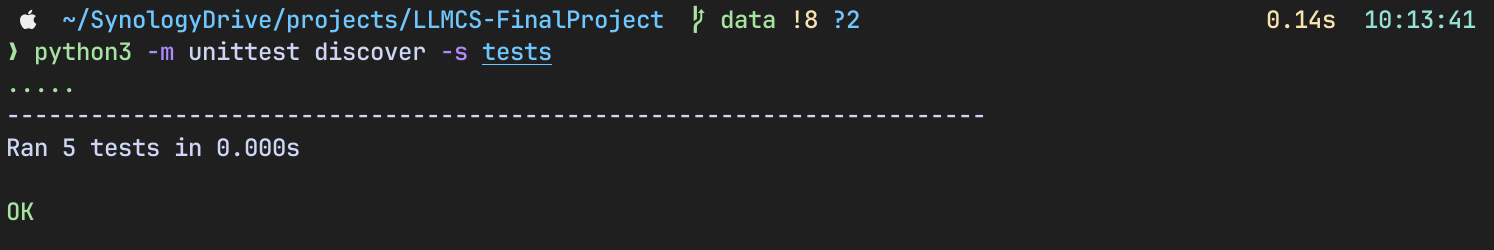
\includegraphics[width=0.72\linewidth]{screenshots/data_week15_tests.png}
  }{
    \fbox{\parbox{0.9\linewidth}{Screenshot placeholder: terminal output from \texttt{python3 -m unittest discover -s tests}.}}
  }
}
\caption{Week 15 evaluation metric unit tests.}
\end{figure}

\section{Week 16 handoff}

The next step is to run the clean dataset and attack set through the completed n8n/LLM workflow and save prediction records. The expected fields are \texttt{message\_id}, \texttt{expected\_label}, \texttt{predicted\_label} or \texttt{label}, \texttt{confidence}, \texttt{final\_action}, and \texttt{validation\_status}. With those fields, the current metric helpers can calculate accuracy, malicious recall, normal false positive rate, manual review rate, and attack success rate.


\subsection{Prediction record contract}

For Week 16, prediction records should preserve the original \texttt{message\_id} so model outputs can be joined back to this dataset. A minimal prediction record should look like this:

\begin{lstlisting}[caption={Future prediction record shape for metric calculation.}]
{
  "message_id": "malicious-014",
  "expected_label": "malicious",
  "predicted_label": "malicious",
  "confidence": 0.91,
  "final_action": "quarantine",
  "validation_status": "valid"
}
\end{lstlisting}

This keeps the data-track output independent from the n8n implementation while still making the final metrics reproducible.

\section{Current limitations}

This Week 15 report does not include live n8n or Ollama results. That is intentional for my track: the dataset and evaluation code are ready for integration, but workflow execution and prompt/model behavior belong to the n8n and LLM tracks. The main limitation is that the dataset is synthetic, so final reporting should clearly distinguish synthetic coverage from real-world email diversity.

\section{Reflection}

The main improvement from Week 14 to Week 15 is coverage. Week 14 proved that the data format and validation path worked. Week 15 adds enough examples and attack categories to support meaningful integration testing. The attack set also includes benign injection-like messages, which is important because a useful classifier should resist prompt injection without automatically treating every mention of an attack phrase as malicious.

\end{document}
